\documentclass[a4paper, 11pt]{ctexart}
\usepackage[left=2.5cm, right=2.5cm, top=2.5cm, bottom=2.5cm]{geometry} 
\usepackage{graphicx}
\usepackage{xcolor}
\usepackage{titlesec}
\usepackage{enumitem}
\usepackage{float}

\definecolor{colorPrimary}{HTML}{0052CC}
\definecolor{colorBg}{HTML}{F0F7FF}

\setlength{\parindent}{0pt} 
\setlength{\parskip}{0.5em}
\setlist[itemize]{itemsep=0.2em, topsep=0.2em}

\begin{document}

\begin{center}
    \LARGE\textbf{算法计量与验证实验报告}\\[1em]
    \large 姓名： \quad 学号：
\end{center}

\vspace{2em}

\textbf{运行环境说明}
\begin{itemize}
\item \textbf{操作系统：}macOS
\item \textbf{python版本：}3.13.2
\item \textbf{代码仓库：}https://github.com/maidou07/dsa2026.git
\end{itemize}

\section*{I：验证list的按索引取值为O(1)}

\subsection*{代码}
\begin{figure}[H]
    \centering
    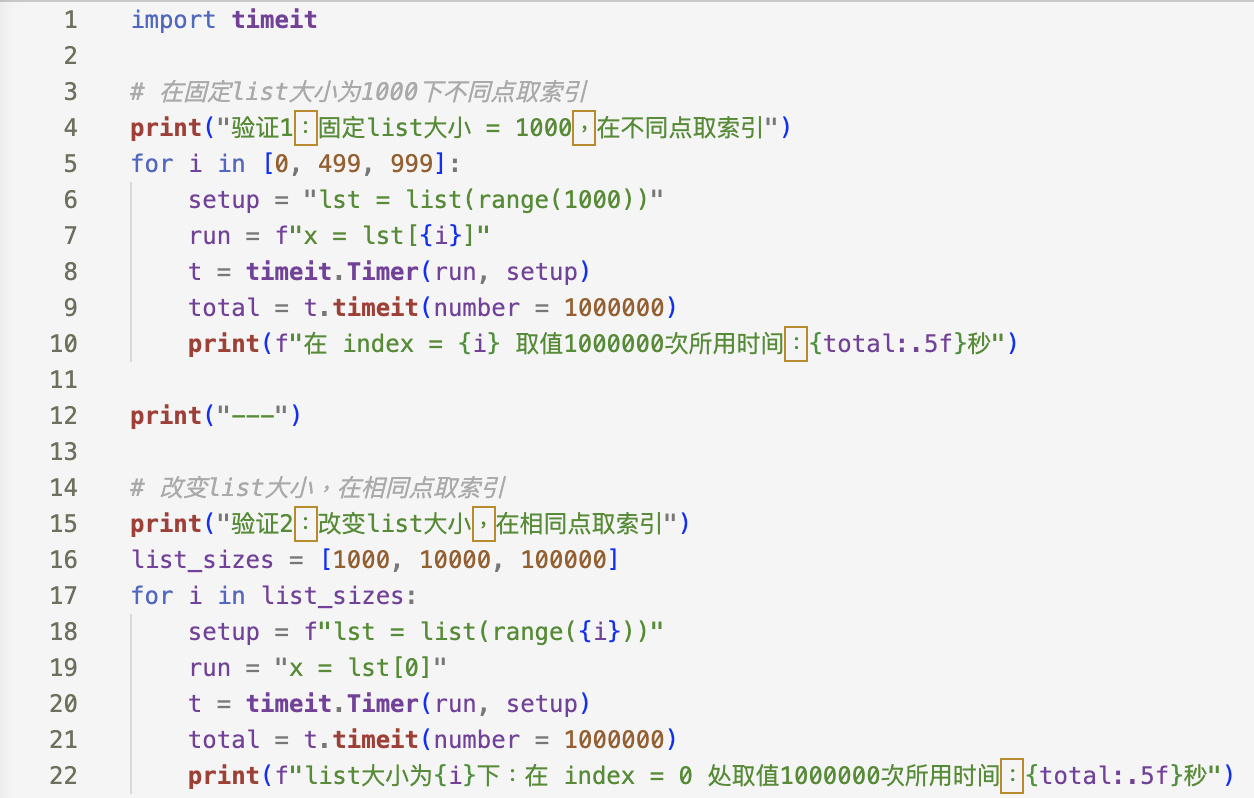
\includegraphics[width=0.9\textwidth]{../img/code0201.png}
\end{figure}

\subsection*{数据说明}
选择两个方面进行完整详细验证:
\begin{itemize}
    \item 一方面固定\texttt{list}的大小，在\textbf{不同索引位置}进行取值操作，选取\texttt{list}大小为1000，在头、中、尾（0，499，999）取值
    \item 另一方面固定在0处取值，\textbf{改变list大小}（1000，10000，100000）
\end{itemize}

\subsection*{运行实验说明}
代码通过\texttt{timeit}计时，并取值1000000次，输出总用时以减小单次调用的时间涨落。

\subsection*{实验结果分析}
\textbf{实验结果}
\begin{verbatim}
验证1：固定list大小 = 1000，在不同点取索引
在 index = 0 取值1000000次所用时间：0.00492秒
在 index = 499 取值1000000次所用时间：0.00495秒
在 index = 999 取值1000000次所用时间：0.00488秒
---
验证2：改变list大小，在相同点取索引
list大小为1000下：在 index = 0 处取值1000000次所用时间：0.00464秒
list大小为10000下：在 index = 0 处取值1000000次所用时间：0.00487秒
list大小为100000下：在 index = 0 处取值1000000次所用时间：0.00447秒
\end{verbatim}

\textbf{分析}

可以看到，在不同大小的\texttt{list}的不同位置取值，所用的时间都基本相同，说明算法的运行时间不依赖于取值位置以及\texttt{list}的大小$N$，故 \texttt{list} 按索引取值的操作时间复杂度为 O(1)。


\vspace{1em} 
\section*{II:验证dict的get item和set item都是O(1)的}

\subsection*{代码}
\begin{figure}[H]
    \centering
    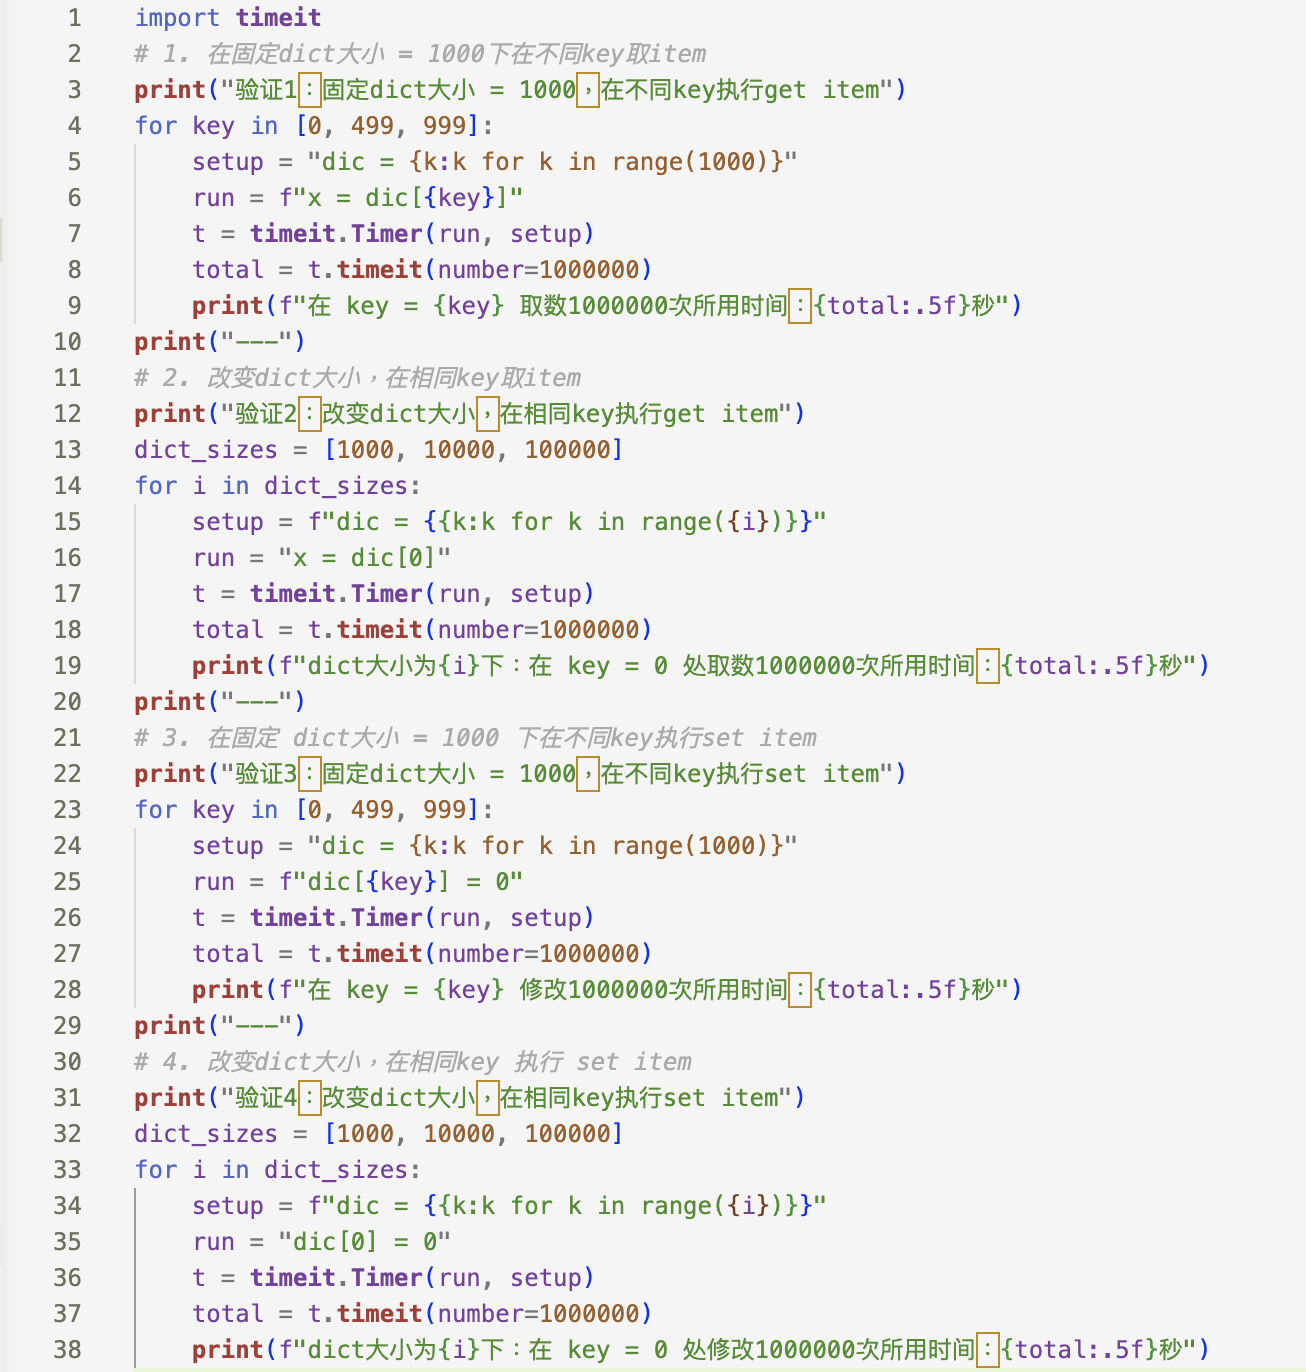
\includegraphics[width=0.9\textwidth]{../img/code0202.png}
\end{figure}

\subsection*{数据说明}
我们每次将\texttt{dict}初始化为\texttt{\{key=k: value=k\}}.
然后使用和I相同的方式，分别对\texttt{get item}和\texttt{set item}都进行了两方面的测试：
\begin{itemize}
    \item \textbf{不同键位置的测试：} 固定\texttt{dict}大小为1000，分别在key为0、499、999处进行读写操作。
    \item \textbf{改变dict大小的同键测试：} 设置\texttt{dict}大小分别为1000、10000、100000，统一对\texttt{key}为0的位置进行读写操作。
\end{itemize}

\subsection*{运行实验说明}
借助 \texttt{timeit.Timer} 模块，对 \texttt{dic[key]} (读取) 和 \texttt{dic[key] = 0} (赋值) 这两条核心语句分别循环执行 $1,000,000$ 次，记录总耗时以减小单次调用的时间涨落。

\subsection*{实验结果分析}
\textbf{实验结果}
\begin{verbatim}
验证1：固定dict大小 = 1000，在不同key执行get item
在 key = 0 取数1000000次所用时间：0.00637秒
在 key = 499 取数1000000次所用时间：0.01106秒
在 key = 999 取数1000000次所用时间：0.01096秒
---
验证2：改变dict大小，在相同key执行get item
dict大小为1000下：在 key = 0 处取数1000000次所用时间：0.00624秒
dict大小为10000下：在 key = 0 处取数1000000次所用时间：0.00643秒
dict大小为100000下：在 key = 0 处取数1000000次所用时间：0.00647秒
---
验证3：固定dict大小 = 1000，在不同key执行set item
在 key = 0 修改1000000次所用时间：0.01007秒
在 key = 499 修改1000000次所用时间：0.01288秒
在 key = 999 修改1000000次所用时间：0.01229秒
---
验证4：改变dict大小，在相同key执行set item
dict大小为1000下：在 key = 0 处修改1000000次所用时间：0.00941秒
dict大小为10000下：在 key = 0 处修改1000000次所用时间：0.00927秒
dict大小为100000下：在 key = 0 处修改1000000次所用时间：0.00969秒
\end{verbatim}

\textbf{分析}

1. 当数据量级发生改变时，操作时间仍基本相同。这证明了基于Hash表实现的字典能够以$O(1)$复杂度完成寻址和修改操作。

2. \textbf{关于 \texttt{key=0} 耗时异常偏低的讨论：} 
由于 Python 底层优化 —— Python的\textbf{小整数缓存池}机制，程序预先缓存了$[-5,256]$的小整数对象，导致\texttt{key=0} 耗时异常偏低。\\
但是可以看到其余 \texttt{key} 耗时基本相同，说明算法总体趋势依然严格遵循 $O(1)$ 的时间复杂度模型。

\vspace{1em} 
\section*{III: 比较 \texttt{list} 和 \texttt{dict} 的 \texttt{del} 操作时间复杂度}

\subsection*{代码}
\begin{figure}[H]
    \centering
    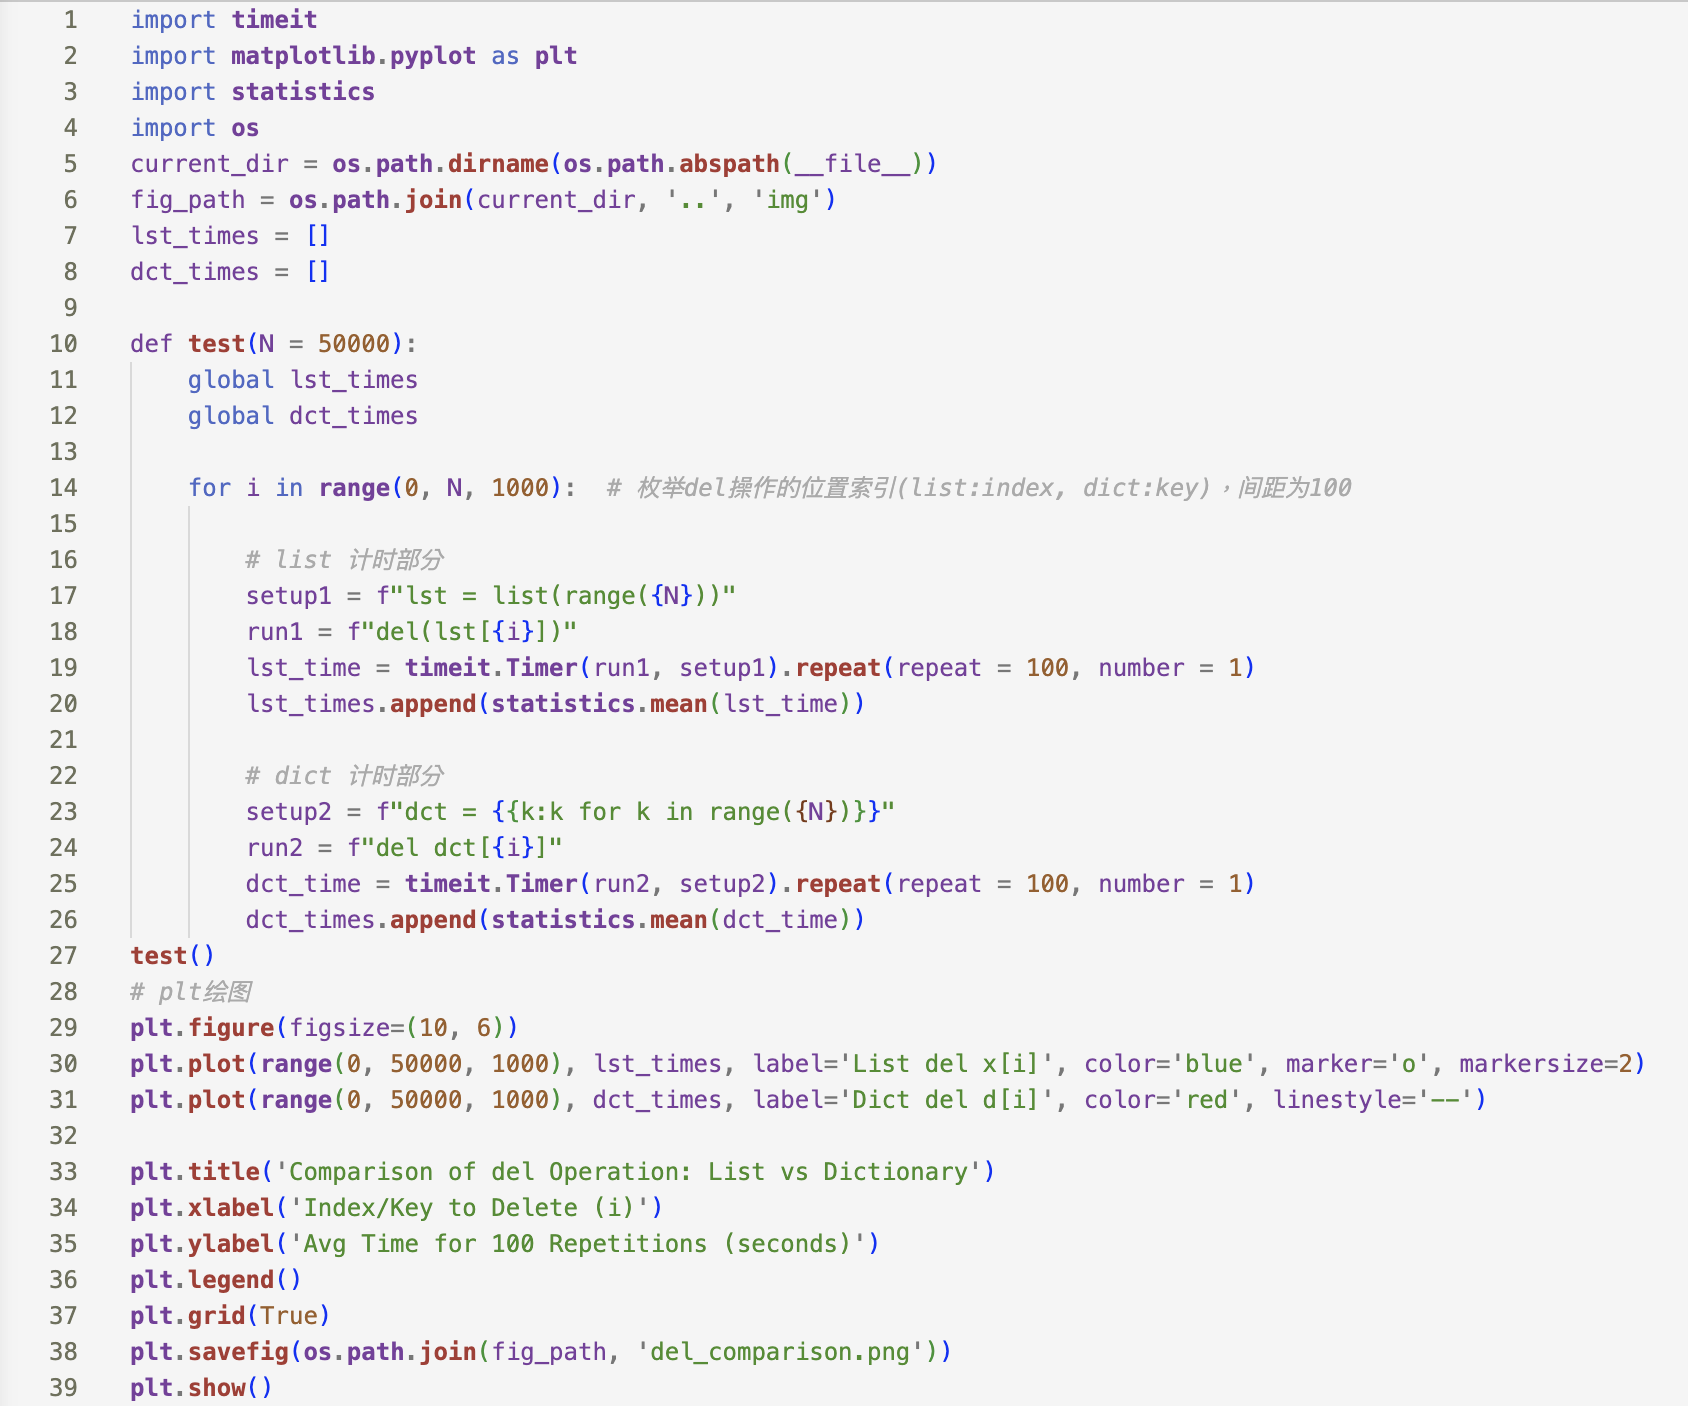
\includegraphics[width=0.9\textwidth]{../img/code0203.png}
\end{figure}

\subsection*{数据说明}
预先构造包含 50000 个元素的 list 和 dict。在 $0$ 到 $50000$ 的索引（或键）范围内，以 1000 为步长，分别枚举并删除对应位置的元素。

\subsection*{运行实验说明}
考虑到 \texttt{del} 操作的不可逆性，实验在 \texttt{setup} 阶段每次都重新生成完整的测试结构。对于每个选定的删除位置 $i$，重复执行 100 次 \texttt{del} 并利用 \texttt{statistics.mean()} 求取平均耗时。最后通过 \texttt{matplotlib} 将得到的数据点绘制成对比折线图。

\subsection*{实验结果分析}
\textbf{实验结果}：

\begin{figure}[H]
    \centering
    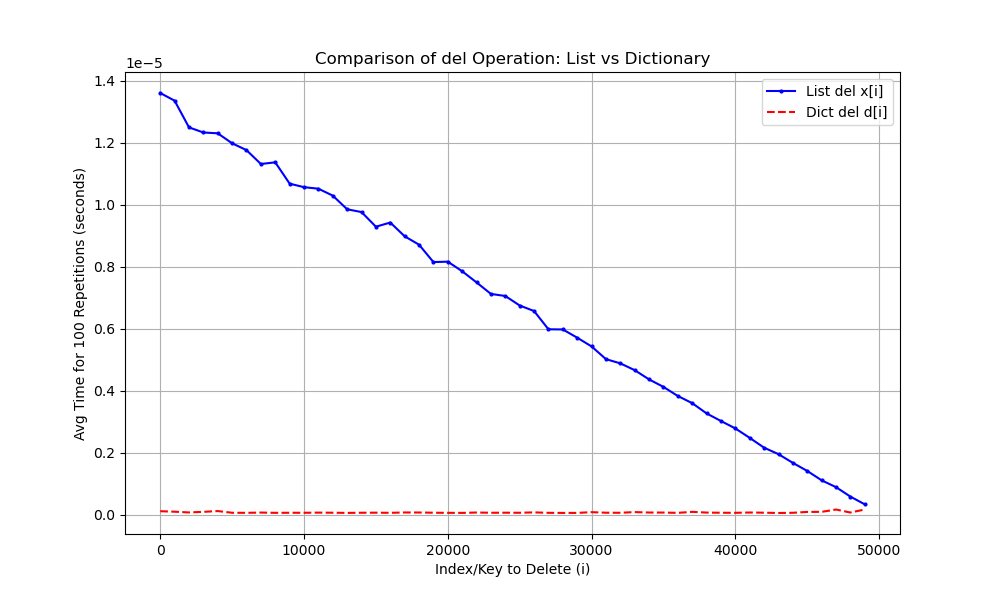
\includegraphics[width=0.9\textwidth]{../img/del_comparison.png}
\end{figure}

\textbf{分析}：
从绘制的耗时折线图可以直观地得出以下结论：
\begin{itemize}
    \item \textbf{对于 dict（红色虚线）：} \texttt{del} 操作的耗时几乎贴近 X 轴并保持水平，完全不随被删除元素所处位置的变化而改变。这印证了字典的 \texttt{del} 也是通过哈希定位，时间复杂度为 $O(1)$。
    \item \textbf{对于 list（蓝色实线）：} 耗时呈现出明显的\textbf{线性下降趋势}。这是由于 Python 的 \texttt{list} 在底层由连续内存的数组实现，当删除索引为 $k$ 的元素时，必须将其后方 $N - 1 - k$ 个元素整体向前移动一位。因此，当 $k$ 越小（越靠近列表头部），需要移动的元素越多，耗时最长，整体呈现 $O(N)$ 的复杂度特性；当 $k$ 靠近尾部时，无需移动其他元素，耗时逐渐逼近 $O(1)$，故\texttt{list}的\texttt{del}操作可以总结为 $O(N-k)$ 的时间复杂度。
\end{itemize}


\vspace{1em} 
\section*{IV: 验证 \texttt{list.sort()} 的时间复杂度为$ O(N \log N)$}

\subsection*{代码}
\begin{figure}[H]
    \centering
    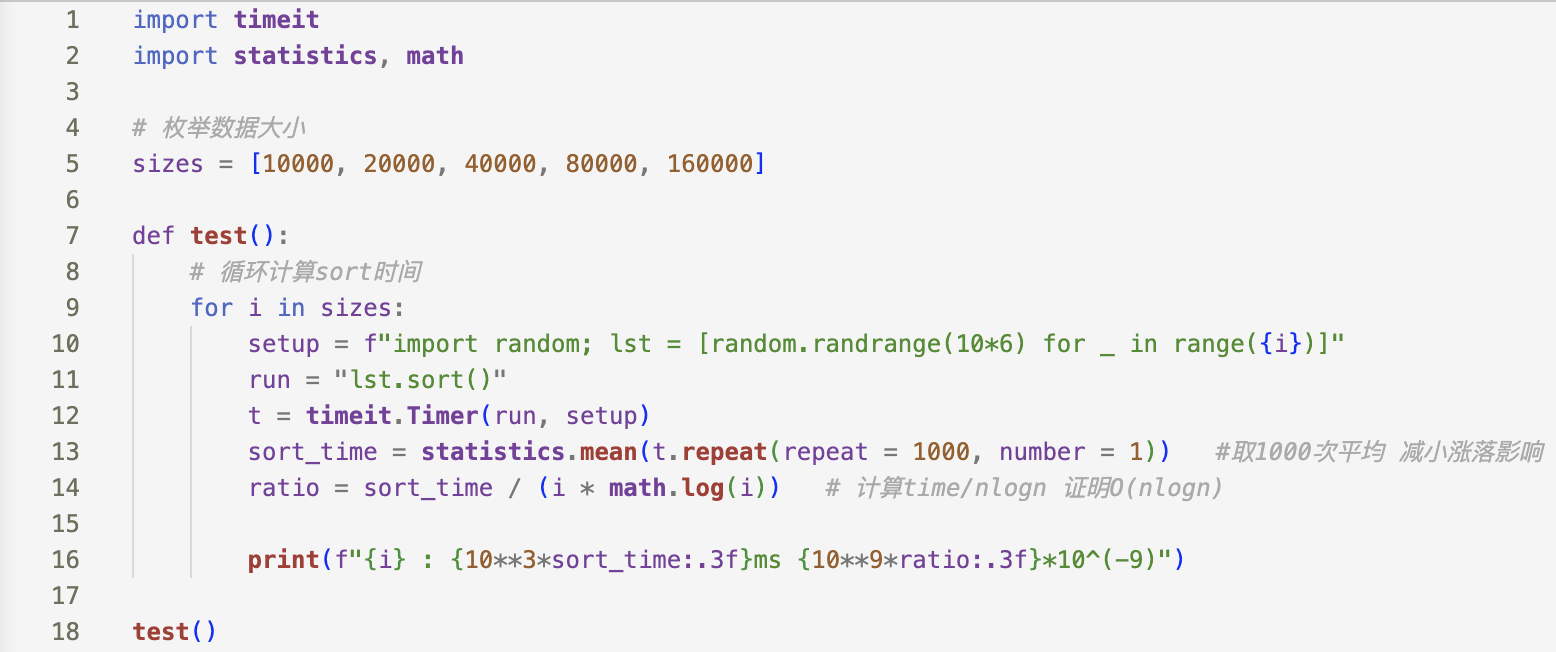
\includegraphics[width=0.9\textwidth]{../img/code0204.png}
\end{figure}

\subsection*{数据说明}
枚举不同的数据规模：$10000, 20000, 40000, 80000, 160000$。针对每种规模，利用 \texttt{random} 模块生成完全无序的随机整数列表。

\subsection*{运行实验说明}
由于 \texttt{sort()} 算法在排序之后，再次排序的时间复杂度会退化，因此在 \texttt{timeit} 的 \texttt{setup} 中必须每次都重新生成无序数组。实验对每种规模重复执行 1000 次求得平均时间 $t$。\\

为了验证其是否符合 $O(N \log N)$ 的规律，我们计算了比值 $ratio = \frac{t}{N \log N}$。 如果时间复杂度符合该模型，则比值应趋近于一个常数。

\subsection*{实验结果分析}
\textbf{实验结果}

输出格式为：\\
数据规模 : 用时(ms) ratio\\
\vspace{-2em}
\begin{verbatim}
10000 : 0.446ms 4.839*10^(-9)
20000 : 0.898ms 4.536*10^(-9)
40000 : 1.814ms 4.280*10^(-9)
80000 : 3.667ms 4.061*10^(-9)
160000 : 7.465ms 3.893*10^(-9)
\end{verbatim}

\textbf{分析}

通过代码输出结果可以观察到：尽管数据规模 $N$ 成倍增加，但计算出的比值却基本相同。说明用时$t$与$N \log N$ 存在严格比例关系，验证了 Python 内置的 \texttt{sort()}在处理一般无序数据时，时间复杂度满足 $O(N \log N)$ 模型。

\end{document}